% Options for packages loaded elsewhere
\PassOptionsToPackage{unicode}{hyperref}
\PassOptionsToPackage{hyphens}{url}
%
\documentclass[
]{article}
\title{Simulation study for debiased learning}
\author{}
\date{\vspace{-2.5em}}

\usepackage{amsmath,amssymb}
\usepackage{lmodern}
\usepackage{iftex}
\ifPDFTeX
  \usepackage[T1]{fontenc}
  \usepackage[utf8]{inputenc}
  \usepackage{textcomp} % provide euro and other symbols
\else % if luatex or xetex
  \usepackage{unicode-math}
  \defaultfontfeatures{Scale=MatchLowercase}
  \defaultfontfeatures[\rmfamily]{Ligatures=TeX,Scale=1}
\fi
% Use upquote if available, for straight quotes in verbatim environments
\IfFileExists{upquote.sty}{\usepackage{upquote}}{}
\IfFileExists{microtype.sty}{% use microtype if available
  \usepackage[]{microtype}
  \UseMicrotypeSet[protrusion]{basicmath} % disable protrusion for tt fonts
}{}
\makeatletter
\@ifundefined{KOMAClassName}{% if non-KOMA class
  \IfFileExists{parskip.sty}{%
    \usepackage{parskip}
  }{% else
    \setlength{\parindent}{0pt}
    \setlength{\parskip}{6pt plus 2pt minus 1pt}}
}{% if KOMA class
  \KOMAoptions{parskip=half}}
\makeatother
\usepackage{xcolor}
\IfFileExists{xurl.sty}{\usepackage{xurl}}{} % add URL line breaks if available
\IfFileExists{bookmark.sty}{\usepackage{bookmark}}{\usepackage{hyperref}}
\hypersetup{
  pdftitle={Simulation study for debiased learning},
  hidelinks,
  pdfcreator={LaTeX via pandoc}}
\urlstyle{same} % disable monospaced font for URLs
\usepackage[margin=1in]{geometry}
\usepackage{color}
\usepackage{fancyvrb}
\newcommand{\VerbBar}{|}
\newcommand{\VERB}{\Verb[commandchars=\\\{\}]}
\DefineVerbatimEnvironment{Highlighting}{Verbatim}{commandchars=\\\{\}}
% Add ',fontsize=\small' for more characters per line
\usepackage{framed}
\definecolor{shadecolor}{RGB}{248,248,248}
\newenvironment{Shaded}{\begin{snugshade}}{\end{snugshade}}
\newcommand{\AlertTok}[1]{\textcolor[rgb]{0.94,0.16,0.16}{#1}}
\newcommand{\AnnotationTok}[1]{\textcolor[rgb]{0.56,0.35,0.01}{\textbf{\textit{#1}}}}
\newcommand{\AttributeTok}[1]{\textcolor[rgb]{0.77,0.63,0.00}{#1}}
\newcommand{\BaseNTok}[1]{\textcolor[rgb]{0.00,0.00,0.81}{#1}}
\newcommand{\BuiltInTok}[1]{#1}
\newcommand{\CharTok}[1]{\textcolor[rgb]{0.31,0.60,0.02}{#1}}
\newcommand{\CommentTok}[1]{\textcolor[rgb]{0.56,0.35,0.01}{\textit{#1}}}
\newcommand{\CommentVarTok}[1]{\textcolor[rgb]{0.56,0.35,0.01}{\textbf{\textit{#1}}}}
\newcommand{\ConstantTok}[1]{\textcolor[rgb]{0.00,0.00,0.00}{#1}}
\newcommand{\ControlFlowTok}[1]{\textcolor[rgb]{0.13,0.29,0.53}{\textbf{#1}}}
\newcommand{\DataTypeTok}[1]{\textcolor[rgb]{0.13,0.29,0.53}{#1}}
\newcommand{\DecValTok}[1]{\textcolor[rgb]{0.00,0.00,0.81}{#1}}
\newcommand{\DocumentationTok}[1]{\textcolor[rgb]{0.56,0.35,0.01}{\textbf{\textit{#1}}}}
\newcommand{\ErrorTok}[1]{\textcolor[rgb]{0.64,0.00,0.00}{\textbf{#1}}}
\newcommand{\ExtensionTok}[1]{#1}
\newcommand{\FloatTok}[1]{\textcolor[rgb]{0.00,0.00,0.81}{#1}}
\newcommand{\FunctionTok}[1]{\textcolor[rgb]{0.00,0.00,0.00}{#1}}
\newcommand{\ImportTok}[1]{#1}
\newcommand{\InformationTok}[1]{\textcolor[rgb]{0.56,0.35,0.01}{\textbf{\textit{#1}}}}
\newcommand{\KeywordTok}[1]{\textcolor[rgb]{0.13,0.29,0.53}{\textbf{#1}}}
\newcommand{\NormalTok}[1]{#1}
\newcommand{\OperatorTok}[1]{\textcolor[rgb]{0.81,0.36,0.00}{\textbf{#1}}}
\newcommand{\OtherTok}[1]{\textcolor[rgb]{0.56,0.35,0.01}{#1}}
\newcommand{\PreprocessorTok}[1]{\textcolor[rgb]{0.56,0.35,0.01}{\textit{#1}}}
\newcommand{\RegionMarkerTok}[1]{#1}
\newcommand{\SpecialCharTok}[1]{\textcolor[rgb]{0.00,0.00,0.00}{#1}}
\newcommand{\SpecialStringTok}[1]{\textcolor[rgb]{0.31,0.60,0.02}{#1}}
\newcommand{\StringTok}[1]{\textcolor[rgb]{0.31,0.60,0.02}{#1}}
\newcommand{\VariableTok}[1]{\textcolor[rgb]{0.00,0.00,0.00}{#1}}
\newcommand{\VerbatimStringTok}[1]{\textcolor[rgb]{0.31,0.60,0.02}{#1}}
\newcommand{\WarningTok}[1]{\textcolor[rgb]{0.56,0.35,0.01}{\textbf{\textit{#1}}}}
\usepackage{graphicx}
\makeatletter
\def\maxwidth{\ifdim\Gin@nat@width>\linewidth\linewidth\else\Gin@nat@width\fi}
\def\maxheight{\ifdim\Gin@nat@height>\textheight\textheight\else\Gin@nat@height\fi}
\makeatother
% Scale images if necessary, so that they will not overflow the page
% margins by default, and it is still possible to overwrite the defaults
% using explicit options in \includegraphics[width, height, ...]{}
\setkeys{Gin}{width=\maxwidth,height=\maxheight,keepaspectratio}
% Set default figure placement to htbp
\makeatletter
\def\fps@figure{htbp}
\makeatother
\setlength{\emergencystretch}{3em} % prevent overfull lines
\providecommand{\tightlist}{%
  \setlength{\itemsep}{0pt}\setlength{\parskip}{0pt}}
\setcounter{secnumdepth}{-\maxdimen} % remove section numbering
\usepackage{statstyle}
\ifLuaTeX
  \usepackage{selnolig}  % disable illegal ligatures
\fi

\begin{document}
\maketitle

\hypertarget{simulation-setup}{%
\section{Simulation setup}\label{simulation-setup}}

Let \(A\) be a sample of size \(n =\) 100 selected from the population
\(U\) of size \(N =\) 2000. Let \(y\) be a variable of interest and we
try to estimate the population total \(t_y = \sum_{i \in U} y_i\) and
\(\bf x_{i}\) of size \(p\) be the auxiliary variables associated with
\(y\) where \(x_{ij} \iid N(2, 1)\). Suppose the following
superpopulation model holds \[
y_i = \bf x_i^T \bf \beta + \varepsilon_i, \quad \varepsilon_i \iid N(0,\sigma^2), i = 1, \cdots, N
\] where \(\sigma^2 = 1\) and
\(\bf \beta = (1, \cdots, 1, 0, \cdots, 0)\) with \(s =\) 20 1s and
\(p - s =\) 20 0s. We assume the samples are drawn from the informative stratified sampling.

    $$
    Z_j \sim Z_j^* + \varepsilon_j, \quad Z^* \sim N\pa{0, \frac{1 - r}{r}}, j \in U, r \in (0, 1)
    $$
    The finite population data $\set{y_j, x_j, z_j}_{j \in U}$ are sorted by $z_j$ so that the 500 smallest $z$ values are in stratum one and the next 500 smallest value are in stratum two and so forth. Within each stratum, simple random samples are collected with size
    $$
    n_1 = 15, n_2 = 20, n_3 = 30, n_4 = 35
    $$
The larger $r$ is, the more informative sampling design we have. We consider the following estimators. Here, we set $r = 0.75$.

\begin{itemize}
  \item Difference estimator
  $$
  \hat t_y = \pa{\sum_{i \in U}\bf x_i}^T \bf \beta + \sum_{i \in A} d_i \pa{y_i - \bf x_i^T \bf \beta}
  $$
  \item GREG estimator
  $$
  \hat t_y = \pa{\sum_{i \in U}\bf x_i}^T \hat{\bf \beta} + \sum_{i \in A} d_i \pa{y_i - \bf x_i^T \hat{\bf \beta}}
  $$
  where $\hat {\bf \beta} = \pa{\sum_{i \in A} d_i \bf x_i \bf x_i^T}^{-1} \pa{\sum_{i \in A} d_i \bf x_i y_i}$
  
  \item Model-based estimator
  $$
  \hat t_y = \pa{\sum_{i \in U}\bf x_i}^T \hat{\bf \beta}
  $$
  
  \item Debiased GREG estimator(Proposed)
    $$
  \hat t_y = \pa{\sum_{i \in U}\bf x_i}^T \pa{ \frac{\sum_{i \in A_2}d_i}{\sum_{i \in A}d_i} \hat{\bf \beta}_1 + \frac{\sum_{i \in A_1}d_i}{\sum_{i \in A}d_i} \hat{\bf \beta}_2} + \sum_{i \in A_1} d_i \pa{y_i - \bf x_i^T \hat{\bf \beta}_2} + \sum_{i \in A_2} d_i \pa{y_i - \bf x_i^T \hat{\bf \beta}_1}
  $$
  where $A_1$ and $A_2$ are the subsamples of $A$ with $A_1 \bigcup A_2 = A$, and $\hat {\bf \beta}_1$ and $\hat {\bf \beta}_2$ are the regression coefficients built upon the sample $A_1$ and sample $A_2$ respectively.
  \item Design unbiased GREG estimator(Sande, 2021)
  $$
  \hat t_y = \pa{\sum_{i \in U}\bf x_i}^T \hat{\bf \beta}_1 + \sum_{i \in A_1} \pa{y_i - \bf x_i^T \hat{\bf \beta}_1} + \sum_{i \in A_2} \frac{1}{P(i \in A_2 | i \in A)} \pa{y_i - \bf x_i^T \hat{\bf \beta}_1}
  $$
  
  %\item LASSO estimator
  %\item Debiased Lasso estimator(Zhang \& Zhang, 2014)
\end{itemize}

\begin{Shaded}
\begin{Highlighting}[]
\FunctionTok{cbind}\NormalTok{(BIAS, SE, RMSE)}
\end{Highlighting}
\end{Shaded}

\begin{verbatim}
##                        BIAS       SE     RMSE
## HT              14.17026931 344.5636 344.8548
## Diff            -0.08421959 118.2858 118.2858
## GREG           218.84918216 198.7317 295.6167
## Lasso          161.59757722 181.5888 243.0808
## Debiased         3.79573031 240.6009 240.6309
## Lasso_Debiased  12.38923464 198.2491 198.6358
\end{verbatim}

\begin{Shaded}
\begin{Highlighting}[]
\FunctionTok{library}\NormalTok{(ggplot2)}
\end{Highlighting}
\end{Shaded}

\begin{verbatim}
## Warning: package 'ggplot2' was built under R version 4.0.5
\end{verbatim}

\begin{Shaded}
\begin{Highlighting}[]
\FunctionTok{ggplot}\NormalTok{() }\SpecialCharTok{+} 
  \FunctionTok{geom\_density}\NormalTok{(}\AttributeTok{data =} \FunctionTok{data.frame}\NormalTok{(res), }\FunctionTok{aes}\NormalTok{(}\AttributeTok{x =}\NormalTok{ Diff, }\AttributeTok{fill =} \StringTok{"Diff"}\NormalTok{), }\AttributeTok{alpha =} \FloatTok{0.3}\NormalTok{) }\SpecialCharTok{+}
  \FunctionTok{geom\_density}\NormalTok{(}\AttributeTok{data =} \FunctionTok{data.frame}\NormalTok{(res), }\FunctionTok{aes}\NormalTok{(}\AttributeTok{x =}\NormalTok{ GREG, }\AttributeTok{fill =} \StringTok{"GREG"}\NormalTok{), }\AttributeTok{alpha =} \FloatTok{0.3}\NormalTok{) }\SpecialCharTok{+} 
  \FunctionTok{geom\_density}\NormalTok{(}\AttributeTok{data =} \FunctionTok{data.frame}\NormalTok{(res), }\FunctionTok{aes}\NormalTok{(}\AttributeTok{x =}\NormalTok{ Debiased, }\AttributeTok{fill =} \StringTok{"Debiased"}\NormalTok{), }\AttributeTok{alpha =} \FloatTok{0.3}\NormalTok{) }\SpecialCharTok{+} 
  \FunctionTok{geom\_density}\NormalTok{(}\AttributeTok{data =} \FunctionTok{data.frame}\NormalTok{(res), }\FunctionTok{aes}\NormalTok{(}\AttributeTok{x =}\NormalTok{ Lasso, }\AttributeTok{fill =} \StringTok{"Lasso"}\NormalTok{), }\AttributeTok{alpha =} \FloatTok{0.3}\NormalTok{) }\SpecialCharTok{+} 
  \FunctionTok{geom\_density}\NormalTok{(}\AttributeTok{data =} \FunctionTok{data.frame}\NormalTok{(res), }\FunctionTok{aes}\NormalTok{(}\AttributeTok{x =}\NormalTok{ Lasso\_Debiased, }\AttributeTok{fill =} \StringTok{"Lasso\_Debiased"}\NormalTok{), }\AttributeTok{alpha =} \FloatTok{0.3}\NormalTok{) }\SpecialCharTok{+}
  \FunctionTok{geom\_vline}\NormalTok{(}\AttributeTok{xintercept =}\NormalTok{ t\_y, }\AttributeTok{col =} \StringTok{"red"}\NormalTok{)}
\end{Highlighting}
\end{Shaded}

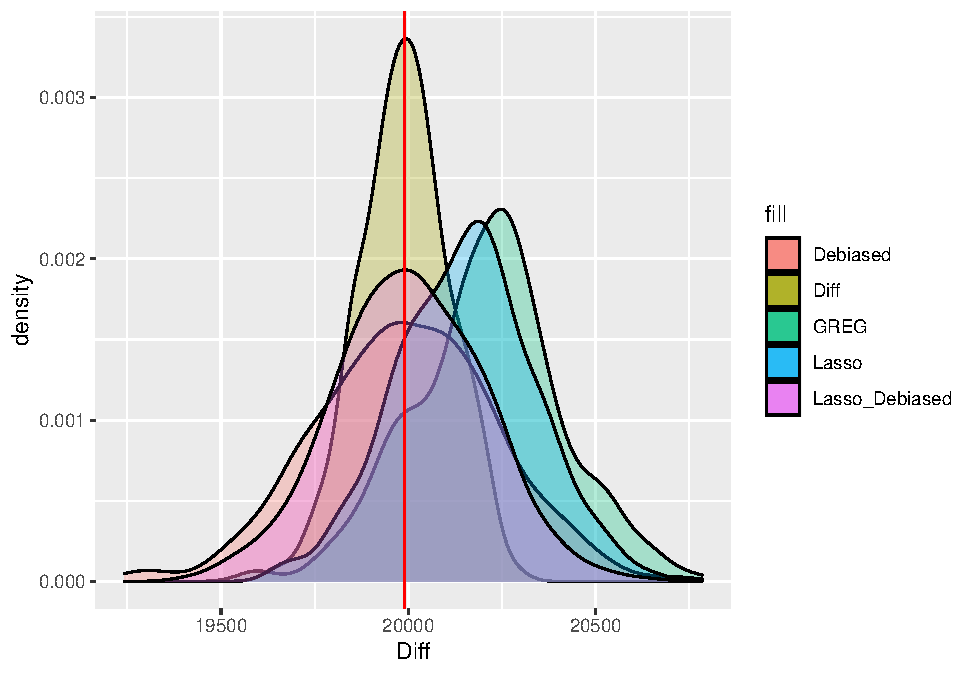
\includegraphics{sim_092922_files/figure-latex/unnamed-chunk-3-1.pdf}



\end{document}
